%% Capitolul 0: INTRODUCERE
%%
%%

\addcontentsline{toc}{chapter}{Introducere}
\markboth{\bf Introducere}{\bf Introducere}

\chapter*{Introducere}
\label{capintro}
\markboth{\bf Introducere}{\bf Introducere}

@Inv@a@tarea automat@a a devenit un subiect de interes din ce @in ce mai important, aceast@a fiind utilizat@a @in vaste domenii, precum: industria auto, alimentar@a, agricol@a, bancar@a, aerospa@tial@a @si mai cu seam@a @in industria tehnologiei informa@tiei. Unul din rolurile ei cele mai importante const@a @in analiza @si clasificarea datelor, predic@tia unor evenimente @in baza unor fapte deja @int@amplate, crearea unui profil virtual pentru un grup de utilizatori, etc.


Datorit@a marei conectivit@a@ti dintre oamenii din ziua de ast@azi; sistemele politice, economice @si rela@tiile interumane au devenit extrem de complexe. Totul a devenit interconectat. O ideea a unui singur individ poate fi transmis@a pe tot globul p@am@antesc, aceasta idee putand afect\^ and milioane de oameni \^ in diverse locuri @si a c\^ arui impact politic @si economic poate fi greu de estimat. De asemenea, un incident economic local, un dezastru natural, sau un conflic politic dintre dou@a @t@ari pot avea efecte devastatoare asupra economiei globale @si a structurii geopolitice curente.

Fiecare eveniment din ziua de ast@azi are o influen@t@a mai mic@a sau mai mare aupra acestei mari re@tele de sisteme ale civiliza@tiei umane. @Intrebarea natural@a la aceast@a dilemna este: putem face o estimare aupra acestor evenimente @si ale cazurilor lor speciale? Se poate, @si asta datorit@a faptului ca multe evenimente sunt monitorizate @si @inregistrate, precum: tranzac@tiile bancare, documente legislative @si juridice, vremea, traseele @si destina@tiile ma@sin@ariilor de transport marf@a (automobile, avioane, vapoare), discursuri @si opinii @in re@tele sociale, date medicale din dispozitive inteligente (telefoane smart, ceasuri @si br@atari smart), date provenite din simul@ari virtuale sau experimente. 

Tot acest mare volum de informa@tii @si metodele de manipulare, stocare @intr@a @in a@sa numita categorie {\sl Big Data}. Analiz@a acestui volum imens de date devine o sarcin@a foarte dificil@a @si laborioas@a @in cazul metodelor conven@tionale de analiz@a a datelor folosind statistic@a clasic@a. @In esen@t@a, @inv@a@tarea automat@a se foloseste at@at de teoria clasic@a c\^  at @si de noile descoperiri @in calculul numeric pentru a crea modele matematice dinamice care pot acumula cuno@tin@te @si ac@tiona @in baza lor folosind toate datele pe care le prime@ste ca set de @inv@a@tare.

\^ In aceast\u a lucrare se va analiza cum algoritmii de @inv@a@tare automat@a  pot fi folosi@ti @in crearea unui agent autonom care s@a @indeplineasc@a sarcinii @intr-un spa@tiu 2-dimensional. Problema const@a @in rezolvarea unui traseu de tip matrice @in care agentul trebuie s@a ajung@a la destina@tie f@ar@a a produce un accident.

Analiza se va face cu ajutorul unei aplica@tii web interactive @in care vom simula mediul nostru 2-dimensional reprezentat de un labirint @si care ne va permite analiza datelor furnizate de c@atre agent @in timpul sesiuni de antrenament pentru determinarea eficien@tei @si fiabilit@a@tii algoritmilor.


\hspace{0.2cm}

@In primul capitol este descris termenul de @inv@a@tare automat@a, care sunt subdomeniile sale, cum este folosit @in @industire. 

@In al doilea capitol este o mic@a introducere pentru re@telele neuronale artificiale.

@In al treilea capitol vor fi prezenta@ti c@a@tiva algoritmi de @inv@a@tare, iar al patrulea descrierea aplica@tiei.

@In al patrulea capitol se va descrie structura aplica@tiei web, a componentelor sale @si modul cum acestea interac@tioneaz@a.

\newpage

%%CAPITOLUL 1
%%
%%
\chapter{ @Inv@a@tare automat@a }
\index{@Inv@a@tare automat@a}

\section{Istoric}
\index{sectiune!S1.1}

	@Inv@a@tarea automat@a este o ramur@a a @inteligen@tei artificiale care se ocup@a cu studiul tehnicilor @si metodelor prin care se ofer@a unui calculator abilitatea de a @inv@a@ta. Prin @inv@a@tare ne referim la posibilitatea de a oferii o decizie @in baza unor cuno@stin@te deduse din experien@te anterioare.

 Multe tehnici din @inv@a@tarea automat@a au la baz@a modelul de interac@tiune al neuronului, descris de c@atre Donal Hebb @in cartea sa {\sl The Organization of Behavior} \cite{donald-hebb-book}. Termenul de @inv@a@tare automat@a (@in englez@a {\sl machine learning}) a aparut @in anul 1953, dat de Arthur Samuel, creatorul unui program de jucat checker, capabil s@a ia decizii bazate pe experien@tele anterioare \cite{arthur-samuel}. @In anul 1957, Frank Rosenblatt creaz@a Perceptron-ul, utilizat @in crearea unui calculatorul capabil s@a recunoasc@a forme @intr-o imagine - folosindu-se de observa@tiile din lucr@arile lui Donald Hebb @si Arthur Samuel. Perceptron-ul de unul singur are o putere destul de limitat@a, dar odat@a cu descoperirea utiliz@arii sale @in combina@tii de mai multe straturi a dat na@stere la termenul de re@tea neuronal@a. 
 
 De-a lungul timpului, acest domeniu a avut o evolu@tie @inceat@a, un factor important find capabilit@a@tile limitate de procesarea ale calculatoarelor. Dar odat@a cu avansurile tehnologice, cercetarea @in acest domeniu a @inceput s@a fie din ce @in ce mai activ@a, @in ultimii ani culmin\^ and cu evenimente care au atras interesului publicului general, precum: IBM's Deep Blue, IBM's Watson, Google's Deepmind @si Google's AlphaGo.
 
 
\newpage

\section{Clasificare}

Fiind un domeniu foarte vast @si cuprinz@ator, aceasta se @imparte @in 3 mari categorii:
\hspace{0.2cm}\begin{itemize}
	\item @Inv@a@tare supervizat@a
	\item @Inv@a@tare nesupervizat@a
	\item @Inv@a@tare prin recompens@a
\end{itemize}

\vspace{0.3cm}
@In @inv@a@tarea supervizat@a, procesul de antrenare se bazeaz@a pe analiza unor date formate din perechi de valori intrare-ie@sire (set de date etichetate) pentru calibrarea func@tiilor de deducere. Este folosit pentru rezolvarea problemelor de clasificare.

Exemple de algoritmi:
\begin{itemize}
	\item Support-vector machines
	\item Regresia liniar@a
	\item Regresia logistic@a
	\item Arbori de decizie
	\item Re@tele neuronale
	\item Clasificator bayesian naiv
\end{itemize}

Pentru @inv@atarea nesupervizat@a, procesul de antrenare const@a @in crearea unor modele interne de recunoa@stere a unor tipare @in urma analizei unui set de date neetichetat. Este deseori folosit @in descoperirea similarit@a@tilor @si diferen@telor @intr-un set de date.

Exemple de algoritmi:
\begin{itemize}
	\item K-means clustering
	\item Autoencoders
	\item Analiza componentei principale
	\item Descompunerea valorilor singulare
\end{itemize}

@In @inv@a@tarea prin recompens@a, procesul de antrenare const@a @in maximizarea unei func@tii de recompens@a, modelul calibr\^ andu-se astfel @incat deciziile luate s@a duc@a spre ob@tinerea unei recompense c\^ at mai mari.

Exemple de algoritmi:
\begin{itemize}
	\item Monte Carlo
	\item Q-learning
	\item SARSA
	\item Deep Q Network
	\item Proximal Policy Optimization
	\item Deep Deterministic Policy Gradient
	\item Trust Region Policy Optimization
\end{itemize}

\section{Industrie}

	Tot mai multe aplica@tii folosesc tehnici de @inv@a@tare automat@a pentru optimizarea produselor, servicilor @si interac@tiunilor cu utilizatorii. Cele mai notabile utiliz@ari fiind:
\begin{itemize}
	\item Algoritimi de c@autare a @stirilor @in baza unor preferin@te oferite explicit sau implicit de catre utilizator.
	\item Reclame personalizate generate dup@a profilele utilizatorilor.
	\item Sisteme de recomand@ari produse.
	\item Etichetarea obiectelor sau persoanelor @in imagini, @inregistr@ari audio sau video.
	\item Sisteme robotice autonome.
	\item Ma@sini autonome.
	\item Sisteme meteorologice
	\item Sisteme de detectare a fraudelor @intr-un sistem bancar.
	\item Clasificare @si predic@tia evenimentelor. 
	\item Optimizarea proceselor de produc@tie a m@arfurilor.
	\item Optimizarea procesului de antrenare pentru atle@ti.
\end{itemize}

	Companiile sunt foarte interesate de modul cum interac@tioneaz@a @si percep clien@tii produselor lor, acestea @incerc\^ and mereu s@a colecteze informa@tii pentru despre modul cum sunt utilizate produsele @in activitatea utilizatorului. Aceste campanii de colectare a datelor au devenit din ce @in ce mai agresiv@a, marile companii software specializate @in re@tele sociale (Facebook, Twitter, Youtube, Linkedin, Reddit) v@and datele utilizatorilor @in vederea oferirii unui profil al consumatorului pentru a stabili interesul pentru produs. Atfel, se poate vinde clientului o reclam@a personalizat@a dup@a preferin@tele sale. 
	 
\section{Programe software pentru dezvoltare}

Interesul puternic pentru acest domeniu a venit @in principal din partea marilor companii software @si hardware, ele dezvolt@and puternice biblioteci pentru procesarea datelor, crearea de re@tele neuronale, algoritmi de @inv@a@tare, etc. Pentru sprijinirea domeniului, aceste unelte sunt oferite dupa ca aplica@tii cu surs@a deschis@a ( @in englez@a {\sl open source} ), av@and o licen@t@a deseori foarte permisibil@a @in vederea utiliz@ari personale @si comerciale.

Calitatea acestor unelte le-a f@acut s@a devin@a un standard @in industrie, at@at comercial@a c\^ at @si academic@a.

Example de biblioteci sau aplica@tii software:

\begin{itemize}
	\item Tensorflow - bibliotec@a dezvoltat@a de c@atre Google @in vederea utiliz@ari cu usurin@t@ a algoritmilor de @inv@a@tare, c@at @si func@tii utilitare pentru manipularea datelor.
	\item PyTorch - bibliotec@a dezvoltat@a de c@atre Facebook pentru protiparea aplica@tilor de viziune computerizate, procesarea limbajului natural, etc.
	\item ML.NET - bibliotec@a dezvoltat@a de Microsoft pentru crearea rapid@a a unor aplica@tii de procesare a datelor folosind algoritmi de @inv@a@tare.
	\item scikit-Learn - bibliotec@a care con@tine func@tii statistice folosite pentru analiza datelor.
	\item Apache Spark - bibliotec@a de aplica@tii destinate pentru procesarea unui volum foarte mare de date.
	\item Apache Kafka - aplica@tie care permite stocarea @si distribuirea unui volum foarte mare de date @in timp real c@atre mai mul@ti consumatori.
	\item Caffe - bibliotec@a pentru dezvoltare aplica@tilor pentru medii de lucru care nu dispun de o putere de procesare foarte mare, precum dispozitivele mobile.
	\item Keras - bibliotec@a pentru dezvoltarea re@telelor neuronale
	\item H2O.ai - platform@a de procesare @si analiz@a a datelor pentru mediul comercial
	
\end{itemize}

\section{Big Data}

O component@a esen@tial@a pentru @inv@a@tarea automat@a este gestionarea datelor care vor fi folosite @si produse de c@atre algoritmi algoritmii @inv@a@tare. Aceast@a gestionare a informa@tiilor, de cele mai multe ori, va intra @in cadrul domeniului de {\sl Big Data }

Conform Uniunii Europene: ,,Big data se refer@a la volume de date colectate at\^ at de mari @si complexe @inc\^ at este nevoie de noi tehnologii, cum ar fi inteligen@t@a artificial@a, pentru a le procesa. Datele provin din nenum@arate surse diferite.''\cite{eu-big-data-definition}

Volumul de date pe care omenirea @il produce cre@ste de la an la an, cea ce face  analiza @si intelegerea datelor s@a fie o sarcin@a din ce @in ce mai dificil@a. Tot mai mul@ti oameni @incep s@a aib@a acces la internet, iar num@arul de dispozitive inteligente (smart phone, smart watch, smarth TV) pe care un individ de dispune cre@ste odat@a cu avansul tehnologic.

Principalele surse de provenien@t@a ale acestor date sunt:
\begin{itemize}
	\item Re@tele sociale - mesaje, imagini create de utilizatori pentru a@si exprima opinia la situa@tia sociala, economic@a @si politic@a - datele pot fi utilizate pentru stabilirea unor tendin@te sociale cu privire la activitatea @si starea emo@tional@a curent@a @si viitoare a oamenilor.
	\item Mediul @si natura - date provenite de la sateli@ti @si senzori pentru monitorizarea schimb@arilor climatice - folosite pentru predic@tia posibilelor dezastre naturale cauzate de activit@a@tile omului.
	\item Sector public - documente, certificate, atestate, adeverin@te emise de c@atre institu@tile publice - pot fi utilizate @in eficientizarea servicilor publice.
	\item Transport - date colectate prin GPS @si de la diferi@ti operatori @in domeniul transportului (transportul public, aeroporturi, g@ari) - pentru optimizarea rutelor @si a curselor de transport.
	\item Sector Medical - fi@se medicale ale pacien@tilor - monitorizarea st@arii de s@anatatea a cet@a@teinolor, utile pentru detectarea posibilelor amen@t@ari de tip biologic.
	\item Iternetul Lucrurilor ({\sl Internet of Things}) - date provenite de la diverse aparate, precum: telefon, ceas, televizor, senzor de gaz, sensor de umiditate, camere video, etc. - utilizate la monitorizare activit@a@tii invidului cu scopul de a u@sura anumite sarcini sau pentru a prevenii incidente.
	\item Sector industrial - re@tele industriale de comunica@tii ( senzori, magistrale de teren, re@tele celulare), rapoarte economice - folosite pentru automatizare @si @imbun@at@a@tirea produselor @si a servicilor. 
	\item Sector bancar - tranzac@tii financiare, rapoarte - utilizate pentru detectarea fraudelor bancare, stabilirea ratelor la dob@anzi, @imprumuturi, schimb valutar, etc.
\end{itemize}

Toate aceste benificii sunt importante pentru societatea din ziua de ast@azi, companii mare concureaza pentru crearea de infrastructur@a @si servicii pentru stocarea @si examinarea datelor.

Exemple de servicii:

\begin{itemize}
	\item Amazon Web Services - cel mai mare furnizor de servicii @si infrastructur@a cloud din lume (av\^ and peste 200 de solu@tii software).
	\item Microsoft Azure 
	\item Google Cloud Platform
	\item IBM Cloud
	\item Oracle Cloud
	\item Alibaba Cloud
\end{itemize}

	
%%CAPITOLUL 2
%%
%%

\chapter{Re@tele neuronale artificiale}

\index{capitol!C2}
\index{@Inv@a@tare automat@a}

\section{Introducere}

O re@tea neuronal@a artificial@a este un model computa@tional inspirat din structura @si modul de fun@tionare al creierului biologic. Conexiunile dintre neuronii artificiali se asem\^ an@a sinapselor, fiecare neuron se conecteaz@a cu alt neuron prin intermediul unor muchii. Semnalul trimis prin aceste muchii este ponderat de ni@ste parametri numi@ti ponderi sinaptice. Mai mul@ti neuroni grupa@ti formeaza un strat, iar mai multe straturi formeaz@a o re@tea.

Procesul de @inv@a@tare presupune g@asirea unor valori potrivite pentru ponderile sinaptice astfel @inc\^ at procesarea semnalului de intrare s@a ofere rezultatul dorit.


\section{Structur@a}

Structura principal@a al unui neuron artificial este bazat pe modelul Perceptron-ului al lui Donald Hebb, modelul matematic fiind:

$$
	y = \varphi \left( \sum_{k=1}^{n} w_k * x_k + b \right),
$$

\indent unde $x$ este vectorul de intrare ({\sl input vector}), $y$ vectorul de ie@sire ({\sl output vector}), $w$ ponderea sinaptic@a ({\sl weight}), $b$ deplasarea ({\sl bias}) @si $\varphi$ este func@tia de activare sau transfer ({\sl activation function}).

Vectorul de intrare este format din numere reale, aceste numere put\^ and reprezenta: imagini, frecven@te, etichete codificate, valori provenite de la senzori, etc. Ponderile sinaptice au rolul de a cre@ste sau descre@ste puterea semnalului reprezentat de valorile vectorului de intrare. Func@tia de activare preia semnalul ponderat @si ofer@a o valoarea specific@a @in baza acestuia. Deplasarea ajut@a la deplasarea semnalului ponderat pentru o mai bun@a aproximare necesar@a pentru @indeplirea anumitor condi@tii ale func@tiei de activare.

\begin{exemplu}

	Un neuron artificial care ac@tioneaz@a precum o poarta logic@a {\bf SAU}(OR) pentru dou@a numere binare are forma:
$$
	y = \varphi ( x_1 + x_2 - 0.5 )
$$
,unde $x = \{ x_i | x_i \in \{0, 1\} \}$, $y \in \{0, 1\}$, $w_1 = 1$, $w_2 = 1$,$b = -0.5$, iar func@tia de activare este: 
$$
	\varphi ( u ) = \left\lbrace
		\begin{array}{lc}
			1 & u \geq 0 \\
			0 & u < 0
		\end{array}
	\right.
$$
\end{exemplu}

{\bf Verificare}. Pentru $x = [1, 0]$, avem $u = 1 + 0 - 0.5 = 0.5$ @si $y = \varphi(u) = \varphi(0.5) = 1$ (acela@si rezultat @si pentru $x = [0, 1]$ - datorit@a propieta@tii de comutativitate a adun@arii).
Pentru $x = [1, 1]$, avem $u = 1 + 1 - 0.5 = 1.5$ cu $\varphi (u) = \varphi ( 2 ) = 1$. Ultimul caz pentru $x = [0, 0]$, vom avea $u = 0 + 0 - 0.5 = -0.5$ cu $\varphi (-0.5) = 0$.

\begin{observatia}
	F@ar@a func@tia de activare, perceptronul ac@tioneaz@a precum o func@tie liniar@a. Prin utilizarea unei func@tii de activare potrivite, puteam aborda mai u@sor problemele neliniare, precum cele pentru clasificarea datelor @in diverse categorii.
\end{observatia}

Un singur perceptron ofer@a doar o singur@a valoare de ie@sire. Dac@a dorim s@a avem mai multe valori de ie@siri trebuie s@a mai adaug@am perceptroni. Gruparea de neuroni artificiali se nume@ste {\sl strat (layer)}.

Structura unui strat format din perceptroni arat@a astfel @in form@a matriceal@a:

$$
	\begin{bmatrix}
		u_1 \\
		u_2 \\
		\vdots \\ 
		u_n \\
	\end{bmatrix}	
	= 
	\begin{bmatrix}
		w_{11} & w_{12} & \cdots & w_{1n} \\
		w_{21} & w_{22} & \cdots & w_{2n} \\
		\cdots & \cdots & \cdots & \cdots \\
		w_{n1} & w_{n2} & \cdots & w_{nn} \\
	\end{bmatrix}
	\begin{bmatrix}
		x_1 \\
		x_2 \\
		\vdots \\
		x_n \\
	\end{bmatrix}
	+
	\begin{bmatrix}
		b_1 \\
		b_2 \\
		\vdots \\
		b_n
	\end{bmatrix}
$$

$$
\begin{bmatrix}
		y_1 \\
		y_2 \\
		\vdots \\ 
		y_n \\
	\end{bmatrix}	
	=
	\begin{bmatrix}
		\varphi (u_1)\\
		\varphi	(u_2) \\
		\vdots \\
		\varphi (u_n)
	\end{bmatrix}
$$

Rezultatele acestui strat pot fi transmise c\^ atre un alt strat care poate avea o alt@a func@tie de activare, astfel putem crea modele matematice mai complexe. Aceast@a @in@siruire de straturi se nume@ste {\sl re@tea (network)}. Straturile intermediare sunt deseori referite ca {\sl straturi ascunse} (\textsl{hidden layers}). Iar o re@tea cu foarte multe straturi asunse poart@a denumirea de {\sl profund@a (deep)}.

Re@tele pot fi structurate @si sub forma unui graf. Fiecare neuron find repezentat de un nod, iar muchiile grafului sunt conexiunile dintre neuroni. Dac@a graful suport nu con@tine cicluri, spunem c@a este uni-directional - o denumire uzual@a peste acest tip de re@tea este {\sl feed-forward (FF)} (denumire pe care o vom folosii @si @in restul acestei lucr@ari). De asemenea, neuroni pot fi interconecta@ti (graful suport con@tine cicluri), fapt care poate oferii re@telei mai mult@a putere de modelare. Acest tip de re@tea este denumit @in general {\sl recurrent neural network (RNN)}

Re@telele neuronale artificiale pot fi considerate ca find "aproximatori universali"\cite{hornik-nn}: 
\begin{quotation}
	Re@telele feed-forward multistrat sunt,@in condi@tii generale ale func@tiei de activare ascuns@a, aproximatori universali dac@a dispun de un num@ar suficient de unit@a@ti asunse.
\end{quotation}

De-a lungul anilor, au fost create foarte multe tipuri de re@tele neuronale artificiale pentru a servii la rezolvarea de probleme din domenii dificile.

Exemple de tipuri de re@tele:

\begin{itemize}
	\item Feed Forward (FF)
	\item Deep Feed Forward (DFF)
	\item Radial Basis Network (RBF)
	\item Recurrent Neural Network (RNN)
	\item Long/Short Term Memory (LSTM)
	\item Markov Chain (MC)
	\item Deep Convolutional Network (DCN)
	\item Deconvolutional Network (DN)
	\item Support Vector Machine (SVM)
	\item Deep Belief Network (DBN)
\end{itemize}


\begin{figure}[h]
	\centering
	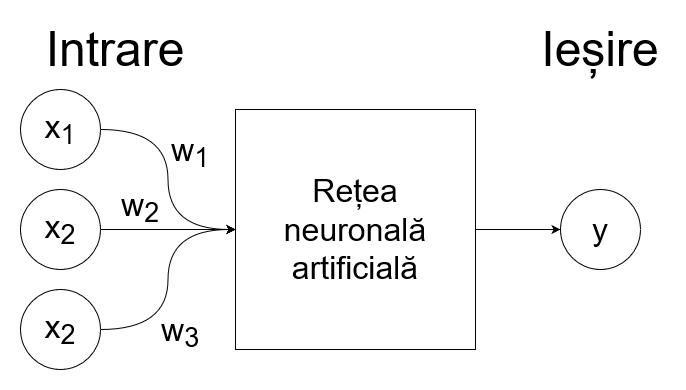
\includegraphics[scale=0.4]{nn_schema_1}
	\caption{Structura unei re@tele neuronale}
	\label{nn:schema}
\end{figure}




\section{Func@tii de activare @si metode de optimizare}
Func@tia de activare ajut@a re@teaua neuronal@a pentru @inv@a@tarea de tipare complexe aflate @in setul de date analizat. Alegerea unei func@tii de activare este critic@a pentru performan@ta re@telei, @in special pentru cazul problemelor neliniare.

Unele din cele mai folosite func@tii sunt:

\begin{align}
	{\rm Identitate} \quad \varphi (x) &= x \\
	{\rm Binary \, Step} \quad \varphi (x) &= \left\lbrace
		\begin{array}{lc}
			1 & x \geq 0 \\
			0 & x < 0
		\end{array}
	\right. \\
	{\rm Logistic, Sigmoid} \quad \varphi (x) &= \displaystyle\frac{1}{1 + e^{-x}} \\
	{\rm Rectified\, liniar\, unit (ReLU)} \quad \varphi (x) &= \left\lbrace
		\begin{array}{lc}
			x & x \geq 0 \\
			0 & x < 0
		\end{array}
	\right. \label{eq:relu} \\
	{\rm Softplus} \quad \varphi (x) &= \ln ( 1 + e^x) 
\end{align}

Func@tiile de activare pot fi aproape orice func@tie liniar@a sau neliniar@a, dar unele  (precum cele enumerate anterior) ofer@a mai multe beneficii dec@at altele @in contextul antren@arii unei re@tele.

Crearea unei re@tele neuronale artificiale presupune alegerea tipurilor de straturi din care s@a fie compus@a @impreun@a cu func@tile lor de activare. La @inceput, ponderile sinaptice sunt de cele mai multe ori alese aleatoriu. Cea ce face ca aproximarea oferit@a de re@tea s@a nu fie una foarte bun@a.

Acest lucru duce la problema de optimizare a re@telei (g@asirea unor valori potrivite pentru ponderile sinaptice) astfel \^inc\^ at rezultatul aproxim@arii s@a fie unul satisf@ac\^ ator. Acest proces este referit uzual ca {\sl antrenare (training)}. Antrenarea este unul dintre cele mai dificile capitole al acestui domeniu, alegerea unui algoritm potrivit poate beneficii extraordinarea @in privin@ta g@asii unor valori optimale pentru ponderile sinaptice.

Re@telele neuronale artificiale folosite @in industrie (aplica@tii de recunoa@stere a obiectelor @in imagini; programe pentru traduceri, recunoa@steri de voce ) au o complexitate extrordinar@a at@at din punct de vedere al arhitecturii, care poate const@a dintr-un mix de diferite tipuri de re@tele, c\^ at @si al nivelului imens de date (de ordinul milioanelor de terabi@ti). Antrenarea acestora poate dura c\^ ateva zile sau c\^ ateva luni, @in cazuri rare fiind vorba de ani. A@sdar, un algoritm de optimizare eficient are un rol crucial @in acest proces.

Ca s@a putem optimiza trebuie s@a avem o metric@a dup@a care s@a evalu@am performan@ta, aceasta poart@a de denumirea de \textbf{func@tie de cost sau pierdere} (\textsl{cost/loss function}). Aceasta se calculeaz@a folosind datele rezultate la rularea re@telei @si cele pe care dorim s@a ale avem. 

@In func@tie de arhitectura re@telei, unele func@tii de cost au o performan@t@a mai bun@a dec\^ at celelalte. C\^ ateva exemple:

\begin{enumerate}
	\item Probleme de regresie
	\begin{enumerate}
		\item Eroarea medie
		\item Eroarea p@atratic@a medie
		\item Eroare medie absolut@a
	\end{enumerate}
	\item Clasific@ari binare
	\begin{enumerate}
		\item Binary Cross-Entropy
		\item Eroare Hinge
		\item Eroare p@atratic@a Hinge
	\end{enumerate}
	\item Clasific@ari multi-clas@a
	\begin{enumerate}
		\item Multi-Class Cross-Entropy
		\item Sparse Multiclass Cross-Entropy
		\item Kullback Leibler Divergence
	\end{enumerate}
\end{enumerate}

S@a presupunem c@a avem tabelul \ref{tab:nn-functie} cu rezultatele unei re@tele care @incerc@a s@a aproximeze urm@atoare func@tie:

\begin{equation} \label{eq:f}
	f:[-1, 1]\rightarrow \mathcal{R}, f(x) = \displaystyle\frac{1}{x^2+1}
\end{equation}

\begin{table}[h]
	\begin{center}
		\begin{tabular}{|c|c|c|}
			\hline
			Date de intrare ($x$) & Rezultat estimat ($\hat{y}$) & Rezultat dorit ($y$) \\
			\hline
			-1 & -1.23 & 0.5 \\
			\hline
			-0.5 & 0.5 & 0.8 \\
			\hline
			0 & 3 & 1 \\
			\hline
			0.5 & -5 & 0.8 \\ 
			\hline
			1 & 0.1 & 0.5 \\ 
			\hline
		\end{tabular}
	\end{center}
	\caption{Valorile estimate pentru func@tia $f(x)$ (\ref{eq:f})}
	\label{tab:nn-functie}
\end{table}

Aplic\^ and eroare medie absolut@a @si eroarea p@atratic@a medie ca func@tii de cost @in tabelul \ref{tab:nn-functie}, ob@tinem urm@atoarele rezultate @in tabelul \ref{tab:nn-erori}\,.

\begin{table}[h]
	\begin{center}
		\begin{tabular}{|c|c|c|}
			\hline
			Func@tie de cost & Formul@a & Valoarea erorii \\
			\hline
			Eroare medie absolut@a & $\displaystyle\frac{1}{n} \sum_{i=1}^{n} |y_i - \hat{y}_i| $ & -1.25 \\
			\hline
			Eroarea p@atratic@a medie & $\displaystyle\frac{1}{n} \sum_{i=1}^{n} \left( y_i - \hat{y}_i \right)^2 $ & 8.18 \\
			\hline
		\end{tabular}
	\end{center}
	\caption{Valorile erorii pentru valorile din tabelul \ref{tab:nn-functie}}
	\label{tab:nn-erori}
\end{table}

Rezultatele ob@tinute din func@tiile cost le putem folosii pentru adjustarea ponderilor sinaptice @si a deplas@arii. Algoritmii care ne ajut@a s@a minimiz@am func@tia de cost ii vom numi \textbf{algoritmi de optimizare}. Pentru re@tele de tip \textsl{Deep Feed Forward (DFF)}, cea mai comun@a metode de adjustare este cea a propag@arii inverse, unde valoarea erorii este transmis@a @in straturile interioare la fiecare neuron. 

Optimizarea re@telei neuronale este unul din cel mai complexe capitole ale domeniului de @inv@a@tare automat@a. Pentru lucrul cu re@tele vom folosii biblioteca Tensorflow, care dispunde de toate cele necesare. Algoritmi de optimizare prezen@ti @in aceast@a bibliotec@a sunt:

\begin{itemize}
	\item Adam
	\item AdaDelta
	\item AdaGrad
	\item AdaMax
	\item Stochastic gradient descent (SGD)
\end{itemize} 

\section{Tensorflow}
Tensorflow este o platform@a dedicat@a dezvolt@arii modelelor de @inv@a@tare automat@a. Acest@a a fost creat@a ini@tial de c@atre Google pentru a accelara dezvoltarea domeniului prin oferirea de programe ajut@atoare pentru crearea rapid@a a protipurilor. Datorit@a calit@atii superioare a programelor de prototipare @si a usurin@tei de utilizare, acesta a devenit o platform@a popular@a at\^ at @in mediul academic c\^ at @si industrial.

Datorit@a popularit@a@tii, platforma a beneficiat de multe contribu@tii importante din partea marilor companii din domeniul IT @si cel al semiconductoarelor, precum: PayPal, AMD, nVIDIA, Blomberg, Intel, IBM, Qualcomm, Uber, Arm, Twitter. De asemenea, platforma beneficieaza de medii interactive de @inv@a@tare, ideale pentru studen@ti sau profesioni@sti care doresc s@a dezvolte mici prototipuri de modele de @inv@a@tare automat@a.

Exemple de programe care fac parte din platforma Tensorflow:
\begin{itemize}
	\item Tensorflow Hub - biblioteca care g@azduie@ste modele predefinite create de comunitate, precum: modele pentru clasificare imaginilor, analiza limbajului natural, generatoare de imagini
	\item Model Optimization - programe dedicate optimiz@arii de modele
	\item TensorFlow Graphics - biblioteca care dispune de unelte pentru procesarea imaginilor
	\item TensorFlow Agents - biblioteca pentru dezolvatare agen@tilor @in cazul @Inv@a@tarii prin recompens@a
\end{itemize}

@In aceasta lucrare vom folosii aceast@a bibliotec@a pentru dezvoltarea unui model pentru agentul care va parcurge labirintul. Unitatea de baz@a pentru lucrul cu aceasta este tensorul, reprezentat prin clasa \texttt{Tensor}. C\^ ateva utliz@arii ale acestei clase pot fi observate @in exempul de cod \ref{lst:exemple-tensor}.

\begin{lstlisting}[language=Java, caption=Exemple de folosire a bibliotecii Tensorflow, label={lst:exemple-tensor}]
// Ini	
import * as tf from "@tensorflow/tfjs";
// Creare a doi tensori 1-dimensionali
const a = tf.tensor1d([1, 2, 3]);
const b = tf.tensor1d([4, 5, 6]);

// Afișarea lor în consolă
a.print(); // [1, 2, 3]
b.print(); // [4, 5, 6]
// Adunare a doi tensori
a.add(b).print(); // [5, 7, 9]

// Crearea unei constante
const k = tf.scalar(5);
// Înmulțirea cu o constantă
a.mul(k).print(); // [5, 10, 15]
// Produsul scalar
a.dot(b).print(); // 32
// Funcția de cost care folosește eroare medie pătratică
tf.losses.meanSquaredError(a, b).print(); // 9
// Crearea unui tensor 2 dimensional
const c = tf.tensor2d([
    [15, 0],
    [80, -30],
]);
// Afișare
c.print(); // [[15, 0  ], [80, -30]]

// Ortogonalizare Gram-Schmidt
tf.linalg.gramSchmidt(c).print(); // [[1, 0 ], [0, -1]]
// Aplicarea funției de activare de ReLU
c.relu().print(); // [[15, 0], [80, 0]]
// Creare unei noi matrici prin adunarea cu un număr
let d = c.add(125);
d.print()
// Extindere ultimei dimensiuni
// Tensorul devine unul 3-dimensional
d = d.expandDims(-1); // [[[140], [125]], [[205], [95 ]]]

// Afișarea formei dimensiunii
console.log(d.shape); // [2, 2, 1]
// Tensorul este este acum de forma unei imaginii
// cu un singur canal de culoare
// Aplicare unei funcții de redimensionare a imaginii
tf.image.resizeBilinear(d, [4, 4]).print();
/*
    [[[140   ],
      [132.5 ],
      [125   ],
      [125   ]],

     [[172.5 ],
      [141.25],
      [110   ],
      [110   ]],

     [[205   ],
      [150   ],
      [95    ],
      [95    ]],

     [[205   ],
      [150   ],
      [95    ],
      [95    ]]]
*/	
\end{lstlisting}


%%CAPITOLUL 3
%%
%%
\chapter{Metode de @inv@a@tare}
\index{capitol!C3}

\section{Lan@t @si proces Markov}

\index{lan@t Markov}
\index{process Markov}

La baza modelului de @inv@atare pe care il vom folosii @in atrenarea agentului stau princiipile fundamentale ale lan@tului Markov @si a procesului Markov.
Propietatea Markov afirm@a c@a viitorul depinde numai de prezent si nu de trecut. Un lan@t Markov este un model probabilistic care depinde numai de starea curenta pentru a prezice o stare viitoare. A@sadar, un lan@t Markov respect@a propietatea Markov.
Trecerea de la o stare la alta se nume@ste tranzi@tie, iar probabilitatea ei poart@a denumirea de probabilitate de tranzi@tie.

De cele mai multe ori, lan@tul Markov este reprezentat sub form@a de graf orientat al c@arui muchii reprezint@a probabilit@a@tile de tranzi@tie dintre varfuri. Suma probailit@a@tilor de tranzi@tie ale unui varf c@atre celelalte varfuri este mereu 1.

In cazul agentului nostru, dac@a ne-am imagina traseul ca find un lan@t Markov, atunci pozi@tiile din trase ar fi varfurile grafului, iar misc@arile agentului ar reprezenta muchiile. Putem asocia fiecarei mi@scare o probabilitate, iar parcurgerea grafului reprezint@a un posibil drum c@atre obiectiv.

A@sadar, dac@a ne-am dorii ca agentul s@a foloseasc@a aceasta idee pentru stabilirea unui drum pentru rezolvarea obiectivului trebuie s@a stabilim o strategie de parcurgere a grafului.
O strategie simpl@a ar fi una de tip {\sl Greddy}, @si anume agentul alege mereu ac@tiunea/muchia cu probabilitatea cea mai mare. Pentru ca aceasta strategie s@a aib@a succes trebuie ca valorile probabilit@atilor act@iunilor s@a conduc@a c@atre obiectiv @in urma parcugerii grafului.

Pentru a controla comportamentul agentului @in mediul de lucru, vom folosii un sistem de recompense pentru fiecare decizie luat@a. Dac@a dorim ca agentul sa evite anumite situa@tii precum luare de ac@tiuni care conduc la coliziuni cu anumite obiecte, vom asocia acestor decizii recompense negative. \^In contrast, dac@a dorim ca agentul s@a fac@a anumite ac@tiuni care duc la \^indeplinirea obiectivelor, acestor decizii li se vor asocia recompense pozitive.

A@sadar, dorim ca pe parcursul simul@arii agentul s@a acumuleze c\^ at mai multe recompense pozitive @si s@a sle evite pe c\^ at mai mult posibil pe cele negative. Acestu lucrul @il vom numi optimizare, iar procesul de antrenament implic@a modificarea re@telei neurale astfel @inc\^ cat ac@tiunile rezultate din datele de intrare s@a maximizeze recompensele acumulate.

Peste lan@tul Markov putem contrui un model matematic pentru modelarea procesului de decizie al agentului. Acest model con@tine urm@atoarele elemente:

\begin{itemize}
	\item Mul@timea st@arilor (S)
	\item Mul@timea ac@tiunilor (A)
	\item Probabilitatea de tranzi@tie dintr-o stare @in alta pentru o ac@tiune ($P(s^{\prime}|s, a)$)
	\item Recompensa primit@a @in urma tranzi@tiei dintr-o stare @in alta pentru o ac@tiune ($R(s^{\prime}|s, a)$)
	\item Factor de atenuare, pondere care exprim@a importan@ta recompenselor imediate @si viitoare ($\gamma$)
\end{itemize}

Recompensele acumulate la fiecare pas de timp sunt exprimate de formula: 
\begin{equation}
	R_t = r_{t+1} + r_{t+2} + ... \,,
\end{equation}


\noindent unde $r_{t+1}$ este recompensa primit@a prin efectuarea unei ac@tiuni la pasul $t_1$. A@sadar, $R_t$ va reprezenta \textbf{c\^ a@stigul}( \textsl{return}), pe care @in mod natural dorim s@a-l maximiz@am. Dar c\^ astigul se poate @intinde pan@a la infinit, ca s@a rezolv@am aceast@a dilema a infinitului, vom introduce @in formul@a factorul de atenuarea ($\gamma$).


\begin{align}
	R_t & =  r_{t+1} + \gamma r_{t+2} + \gamma^{2} r_{t+3} + \gamma^{3} r_{t+4} + ... \\
	& =  r_{t+1} + \gamma \left( r_{t+2} + \gamma r_{t+3} + \gamma^{2} r_{t+4} + ...  \right) \\
	& =  r_{t+1} + \gamma R_{t+1} \\
\end{align}

Factorul de atenuare ar@at@a c\^ at de importante sunt recompensele pentru efectuarea unei strategii cu c\^ a@stig pe termen lung sau scurt. Acest factor ia valori @intre 0 @si 1. Valoriile mai apropiate de 0, dau mai mult@a prioritate ac@tiunilor care ob@tin recompense mari imediate, ignorand ac@tiunile mai slabe, dar care pot avea un c\^ a@stig mare pe o perioada mai lung@a de timp. Pentru valorile mai apropiate de 1, ac@tiunile care duc la un c\^ a@stig mai mare pe perioade lungi vor fi mai importante.

Dac@a am avea un agent pe post de v\^ anz@ator, un factor de atenuare mic ar face ca agentul s@a v{\c a}nd@a produsele c\^ at mai repede la pre@tul curent cel mai mare. Un factor de atenuare mare ar schimba complet strategiea, @si anume c@a agentul va as@tepta s@a v\^ and@a la cel bun pre@t posibil dintr-o perioada de timp. Dac@a am face o lichidare de stoc, atunci v{\c a}anzarea produselor c\^ at mai rapid@a ar avea prioritatea, deci agentul ar trebuii s@a aleag@a recompensele imediate. Pentru v{\c a}nz@ari de produse care @i@si cre@sc valoarea @in timp; precum operele de art@a, imobiliare, titluri financiare (ac@tiuni, obliga@tiuni) - am dorii ca agentul s@a a@stepte un pre@t bun de v\^ anzare.

Pentru alegerea unei ac@tiuni, vom stabilii o \textbf{strategie} $\pi$ (\textsl{policy}), care este o func@tie ce returneaz@a ac@tiunea pe care trebuie s@a o ia agentul la o anumit@a stare. A@sadar, avem $\pi: S \rightarrow A, \pi(s) = a $ pentru $ s \in S, a \in A$.

Fiecarei st@ari @ii putem asocia o \textbf{func@tie valoare} (\textsl{function value}) $V(s)$, valoarea dat@a de aceasta ne va arat@a c\^ at de bun@a este starea @in care se afl@a agentul. Pentru o strategie $\pi$, aceasta are forma:


\begin{align}
	V^{\pi}(s) & =   E_{\pi} \left[ R_t | s_t = s \right] \\
	& =  E_{\pi} \left[ r_{t+1} + \gamma R_{t+1} | s_t = s, s_{t+1} = s^{\prime} \right] \\
	& =   E_{\pi} \left[ r_{t+1}| s_t = s \right] + \gamma E_{\pi} \left[  R_{t+1} | s_{t+1} = s^{\prime} \right] \\
	& =  E_{\pi} \left[ r_{t+1}| s_t = s \right] + \gamma V^{\pi}(s^{\prime})
\end{align}

\noindent Prin urmare, $V^{\pi}(s)$ va fi c\^ a@stigul a@steptat c\^ and se @incepe din starea $s$, iar ac@tiunile sunt date de c\^atre strategia $\pi$.

S@a presupunem c@a avem un magazin @si dorim s@a stabilim pre@tul unui produs pentru o anumit@a zi. Definim starea ca find perechea dintre zi @si pre@t, $S = \left\lbrace  s | s = (zi, pre\c t) \right\rbrace$. Av\^ and o strategie $\pi$ aleatoare, pentru ziua a 5-a, avem urm@atoarele op@tiuni descrise @in tabelul \ref{tab:pret-magazin}.

\begin{table}[h]
	\begin{center}
		\begin{tabular}{|c|c|c|}
			\hline
			Pre@t (lei) & Stare ($s$) & C\^ a@stigul a@steptat ($V^{\pi}(s)$) \\
			\hline
			15 & $s(5,15)$ & 0.3 \\
			\hline
			8 & $s(5,8)$ & 1.6 \\
			\hline
			3 & $s(5,3)$ & 6.9 \\
			\hline
			1 & $s(5,1)$ & 10 \\ 
			\hline
		\end{tabular}
	\end{center}
	\caption{Recompensele a@steptate pentru fiecare pre@t}
	\label{tab:pret-magazin}
\end{table}

Prin scurta analiz@a a tabelului, observ@am c@a agentul decide c@a pre@tul de un leu pentru acel produs va fi cel mai bun. Dac@a am fi luat @in considere @si alte valori pentru reprezentarea st@ari, valori precum: stocul disponibil, rat@a de v\^ anzare zilnic@a, @si am avea acelea@si valori pentru $V^{\pi}(s)$, putem deduce faptul c@a agentul sugereaz@a s@a avem o lichidare de stoc, av\^and @in vedere c@a a ales cel mai mic pre@t.

\section{Q-Learning}

Noi dorim ca agentul s@a ia cele mai bune decizii pentru @indeplinirea sarcinilor, deci am vrea s@a g@asim o strategie optim@a $\pi^*$ @si func@tia valoare optim@a $V^{*}$ care ne ofer@a cel mai mare c\^ a@stig dintre toate celelalte. Metodele de g@asire sunt inspirate din principiul de optimalitatea al lui Richard E. Bellman \cite{bellman-theory}, care afirm@a c@a: ``Strategia optim@a are propietatea c@a indiferent de starea sau decizia ini@tial@a, deciziile care r@am\^ an@a trebuie s@a formeze o strategie optim@a @in ceea ce prive@ste starea rezultat@a din prima decizie``.  

\begin{equation}
	V^{*}(s) = max_{\pi} V^{\pi}(s)
\end{equation}

Pe l@ang@a func@tia valoare $V$, vom avea @si func@tia $Q$ care indic@a c\^ at de bun@a este o ac@tiune pentru o stare av\^and strategia $\pi$. Aceasta este de forma:

\begin{equation}
	Q^{\pi}(s, a) = E_{\pi} \left[ R_t | s_t = s, a_t = a \right]
\end{equation}

Lu\^and exemplul din tabelul \ref{tab:pret-magazin}, putem exemplifica valorile Q prin adaugarea ac@tiunilor: cre@stere pre@t ($\uparrow$), sc@adere pre@t ($\downarrow$) @si p@astrare pre@t ($=$). De asemenea, punem @si condi@tia ca pre@tul s@a nu fie mai mic dec\^at un leu, pentru aceast@a situa@tie nu dorim ca produsul s@a ajung@a s@a fie gratuit.

\begin{table}[h]
	\begin{center}
		\begin{tabular}{|c|c|c|c|}
			\hline
			Pre@t (lei) & Stare ($s$) & Ac@tiune($a$) & Valoare Q ($Q^{\pi}(s, a)$) \\
			\hline
			8 & $s(5,8)$ & $\uparrow$ & -30 \\ 
			\hline
			8 & $s(5,8)$ & $=$ & -10 \\
			\hline
			8 & $s(5,8)$ & $\downarrow$ & 0 \\
			\hline
			3 & $s(5,3)$ & $\uparrow$ & -10 \\ 
			\hline
			3 & $s(5,3)$ & $=$ & 25 \\
			\hline
			3 & $s(5,3)$ & $\downarrow$ & 35 \\
			\hline
			1 & $s(5,1)$ & $\uparrow$ & -30 \\ 
			\hline
			1 & $s(5,1)$ & $=$ & 100 \\
			\hline
			1 & $s(5,1)$ & $\downarrow$ & -120 \\
			\hline
		\end{tabular}
	\end{center}
	\caption{Valorile Q pentru fiecare pre@t @si ac@tiune}
	\label{tab:pret-magazin-q}
\end{table}

Din tabelul \ref{tab:pret-magazin-q} se poate eviden@tia mai detaliat alegerea pre@tului de 1 leu, aceasta av\^and cea mai mare valoare. De asemenea, se pot observa valori negative la ridicarea pre@tului, odat@a cobor\^ at pre@tul, agentul are @sanse mici s@a-l creasc@a. Daca agentul ar fi pornit cu pre@tul din ziua a 4-a, presupun\^ and c@a ar fi cel de 8 lei, @in ziua a 5-a l-ar fi cobor\^ at p\^ an@a la un leu dac@a strategia noastr@a este s@a alegem valoarea Q cea mai mare atunci c\^and decidem ce ac@tiune vom lua. De men@tionat faptul c@a ac@tiunea de cobor\^ are a pre@tului sub un leu are o valoarea extrem de mic@a, asta datorit@a condi@tiei impuse la @inceput. Agentul este complet descurajat s@a ia acea ac@tiune. Aceast@a tactic@a de descurajare o vom folosii @si @in aplica@tie pentru rezolvarea labirintului. Ac@tiunile care fac agentul s@a intre @in obstacole vor avea asociate recompense negative.

Pentru estimarea acestor Q valori vom folosii @inv@a@tarea bazat@a pe diferen@te temporale. Pentru func@tia valoare $V$, aceasta arat@a astfel:

% $$V^{\pi}(s_t) = V^{\pi}(s_t) + \alpha * \left( R_t - V^{\pi}(s_t) \right) = V^{\pi}(s_t) + \alpha * \left( r_{t+1} + \gamma V^{\pi}(s_{t+1})  - V^{\pi}(s_t) \right) ,$$


\begin{align}
	V^{\pi}(s_t) & =  V^{\pi}(s_t) + \alpha * \left( R_t - V^{\pi}(s_t) \right) \\
	 & =  V^{\pi}(s_t) + \alpha * \left( r_{t+1} + \gamma V^{\pi}(s_{t+1})  - V^{\pi}(s_t) \right)
\end{align}

\noindent unde $s_t$ @si $r_t$ sunt starea @si respectiv recompensa la pasul $t$, $\alpha$ este o constant@a numit@a @in general rata de @inv@a@tare (\textsl{learning rate}) @si preiau valori din intervalul 0 @si 1, similar cu factorul de atenuare. $R_t = r_{t+1} + \gamma V^{\pi}(s_{t+1}) $ reprezint@a noua informa@tie, format@a din recompensa imediat@a primit@a la efectuarea ac@tiunii @si c\^ astigul a@steptat pentru urm@toare stare. Diferen@ta dintre aceasta @si valoarea veche reprezint@a valoarea @inv@a@tat@a, iar @inmul@tirea cu constanta $\alpha$ ne arat@a c\^ at prealu@am din aceasta nou@a valuare.

@In mod similar, aplic@am @si pentru valoarea Q:

\begin{align}
	Q^{\pi}(s_t, a_t) & =  Q^{\pi}(s_t, a_t) + \alpha * \left( R_t - Q^{\pi}(s_t, a_t) \right) \\
	 & =  Q^{\pi}(s_t, a_t) + \alpha * \left( r_{t+1} + \gamma Q^{\pi}(s_{t+1}, a_t)  - Q^{\pi}(s_t, a_t) \right)
\end{align}

 De asemenea, definim @si strategia $\varepsilon$-greedy pe care vom folosii @in aplic@tia din aceast@a lucrare, care are urm@atoarele caracteristici:

\begin{itemize}
	\item Ac@tiune din care rezult@a cel mai mare c\^ a@stig estimat este selectat@a.
	\item Av\^ and probabilitatea $\varepsilon$, se alege o ac@tiune @in mod aleatoriu, neglij\^and estimarile pentru recompense.
	\item Pentru echlibrul dintre fazele de explorare @si exploatare a mediului, $\varepsilon$ va @incepe la inceputul simul@arii cu o valoare mare, iar pe parcus, o mic@sor@am p\^ an@a la un minim stabilit.
\end{itemize}

Algoritmul Q-Learning este format din urm@atori pa@sii:

\begin{enumerate}
	\item Se ini@tializeaz@a $Q(s, a)$ @in mod aleatoriu
	\item Ini@tiere episod
	\begin{enumerate}[1.]
		\item Ini@tializare stare $s$
		\item Repet@a
		\begin{enumerate}[1.]
			\item Alegem ac@tiunea $a$ folosind strategia aleas@a (presupunem ca este $\varepsilon$-greedy)
			\item Execut@am ac@tiunea $a$ @si primim recompensa $r$ @si urm@atoarea stare $s^{\prime}$
			\item Actualiz@am valoarea Q a st@arii curente @in func@tie de noile informa@tii: \begin{equation}
			Q^{\pi}(s, a) \leftarrow Q^{\pi}(s, a) + \alpha \left[ r(s,a) + \gamma max_{a^{\prime}} Q^{\pi}(s^{\prime}, a^{\prime}) - Q^{\pi}(s, a) \right]
\end{equation}			
			\item Trecem la urm@atoarea stare: $s = s^{\prime}$
		\end{enumerate}
		\item Repet@am pa@sii pan@a cand se ajunge la o stare terminal@a
	\end{enumerate}	
	\item Repet@am pa@sii at\^at timp c\^ at nu am ajuns la episodul final	
\end{enumerate}

Pentru pasul 2.2.3, $max_{a^{\prime}} Q^{\pi}(s^{\prime}, a^{\prime})$ este recompensa maxim@a ce poate fi ob@tinut@a @in starea $s^{\prime}$ care urmeaz@a st@arii actuale $s$ (recompensa dac@a se ia cea mai bun@a ac@tiune apoi).

%%CAPITOLUL 4
%%
%%
\chapter{Aplica@tie}
\index{capitol!C3}

\section{Introducere}

Pentru aplica@tia @in care vom implementa algoritmit de @inv@a@tare ne dorim s@a avem disponibile urm@atoarele funct@ionalit@a@ti:

\begin{itemize}
	\item Vizualizare grafic@a pentru mediul simulat - Afi@sarea libirintului sub forma unei poze
	\item Grafice pentru analizelor datelor op@tiune din timpul sesiunilor de antrenament
	\item Elemente interactive care s@a ne permit@a modificare de parametri interni @in algoritmi
	\item Tabele care s@a afiseze informa@tii/date care urmeaz@a s@a fie procesate @si rezultatele acestora
\end{itemize}

Av\^ and @in vedere cerin@tele men@tionate anterior, platforma care ne poate permite @in o dezvoltare rapid@a asupra unei interfe@tei interactive foarte bogate este cea a aplicat@ilor destinate web-ului.

Pentru contruirea aplica@tiei vom folosii urm@atoare technologii:

\begin{itemize}
	\item Svelte - program pentru construirea aplica@tilor web care va reprezenta interfa@ta interactiv@a dedicat@a utilizatorului \cite{Svelte}
	\item Tensorflow.js - bibliotec@a dedicat@a pentru contruirea @si antrenarea re@telelor neuronale pentru aplica@tii web \cite{TensorflowJs}
	\item Echarts - bibliotec@a pentru contruirea de graficelor dedicate vizualizarii de date \cite{Echarts}
	\item Konva - bibliotec@a grafic@a pentru generarea imaginilor \cite{Konva}
\end{itemize} 

Elementele de baz@a vor fi construite folosind Svelte, acestea find: butoane, c@ampuri de introducere a datelor, tabele pentru prezentarea informa@tiilor, containere pentru pozi@tionare. Construirea labirintului se va face prin intermediul lui Konva, care ne permite @si modificare rapid@a a imaginii @in func@tie de starea intern@a a simulatorului. Datele provenite din sesiunile de antrenament for fi afi@sate imediat dup@a fiecare sesiune cu ajutorul graficelor generate de Echarts.

Algoritmii de @inv@a@tare vor fi construi@ti folosind func@tile oferite de c@atre Tensorflow, aceastea oferind urm@atoarele capabilit@ati: crearea de straturi cu diverse func@tionalit@a@ti, func@tii de activare, algoritimi de optimizare, metode utilitare de salvare @si de creare a unor modele secven@tiale formate din mai multe straturi de neuroni.

\section{Structur@a}



Labirintul este de forma unei matrici, fiecare celul@a @indepline@ste un anumit rol: drum, obstacol, ie@sire, etc. Clasa principala dedicat@a definirii structurii de reprezentare a la\-bi\-rin\-tului este denumit@a \textbf{Board}. Aceast@a clas@a define@ste mediul simulat @si intereac@tiunile disponibile pentru agent.

Pentru codificare vom avea urm@atoarele reguli: spa@tiul liber va avea cifra 1, un obstacol cifra 2, iar pentru ie@sire cifra 3. Pentru pozi@tile agentului, la codificarea celulei de matrice se va adauga prefixul 1. Exemple de definiri al mediului simulat prin codificare se pot observa @in tabelul~\ref{tab:codific-lab}.


\begin{table}[h]
	\begin{center}
		\begin{tabular}{ccccc}
			\begin{tabular}{|c|c|c|}
				\hline
				11 & 1 & 2 \\
				\hline
				1 & 2 & 2 \\
				\hline
				1 & 1 & 3 \\
				\hline
			\end{tabular} & 
			\begin{tabular}{|c|c|c|}
				\hline
				1 & 1 & 2 \\
				\hline
				11 & 2 & 2 \\
				\hline
				1 & 1 & 3 \\
				\hline
			\end{tabular} &
			\begin{tabular}{|c|c|c|}
				\hline
				1 & 1 & 2 \\
				\hline
				1 & 2 & 2 \\
				\hline
				11 & 1 & 3 \\
				\hline
			\end{tabular} &
			\begin{tabular}{|c|c|c|}
				\hline
				1 & 1 & 2 \\
				\hline
				1 & 2 & 2 \\
				\hline
				1 & 11 & 3 \\
				\hline
			\end{tabular} &
			\begin{tabular}{|c|c|c|}
				\hline
				1 & 1 & 2 \\
				\hline
				1 & 2 & 2 \\
				\hline
				1 & 1 & 13 \\
				\hline
			\end{tabular} \\
		\end{tabular}
	\end{center}
	\caption{Exemple de codific@ari ale structurii labirintului}
	\label{tab:codific-lab}
\end{table}

Sunt disponibile patru ac@tiuni pe care agentul poate s@a le ia: sus, jos, st\^ anga @si dreapta. Ca o ac@tiune s@a fie valid@a, aceasta trebuie s@a @indeplineasc@a urm@atoarea condi@tie: ac@tiunea nu trebuie s@a fac@a agentul s@a ias@a din labirint atunci c\^ and se afl@a la margine. Dac@a se @int\^ ampl@a aces lucru, clasa {\bf Board} va pastra pozi@tia agentului @si va transmitele faptul c@a mutare este invalid@a celorlalte componente astfel @inc\^ at acestea s@a poat@a stabili o recompens@a astfel @inc\^ at ca pe viitor agentul s@a evite astfel de situa@tii.

Reprezentarea libirintului sub form@a de imagine este dat@a de clasa \textbf{BoardUI}. Aceasta are rolul s@a creeze reprezentarea vizual@a a labirintului folosind datele furnizate de c\^ atre clasa \textbf{Board}. Aceast@a reprezentare poate fi observat@a @in figura \ref{fig:labirint-imagine}. Agentul este prezentat sub forma unui cerc albastru, spa@tiul liber sub forma unui p@atrat gri, iar obiectivul cu un p@atrat violet.

\begin{figure}[h]
	\centering
	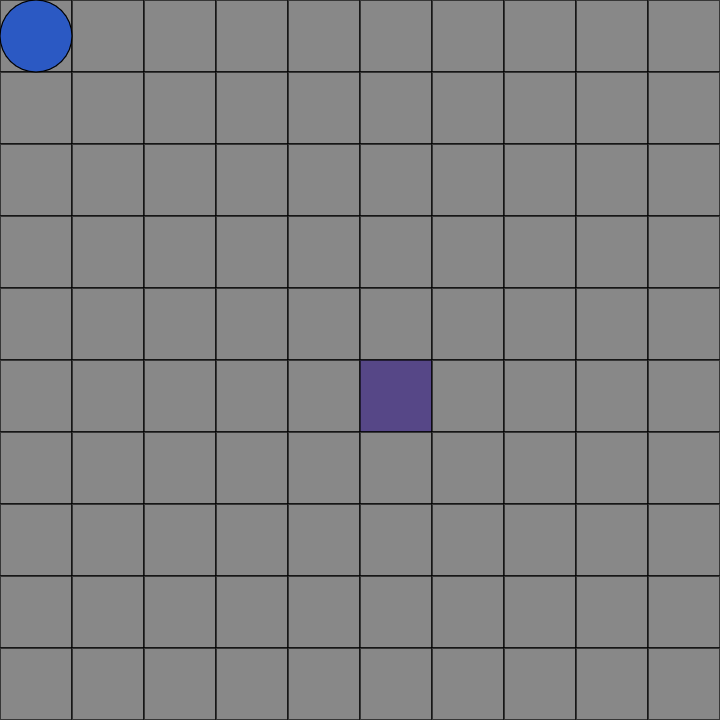
\includegraphics[scale=0.25]{app-labirint-imagine}
	\caption{Reprezentarea vizual@a a labirintului @in starea ini@tial@a}
	\label{fig:labirint-imagine}
\end{figure}

Clas@a \textbf{BoardUI} este legat@a de clasa \textbf{Board} printr-un sistem reactiv de notificare, astfel @inc\^ at orice schimbare care duce la modificarea st@arii labirintului (exemplu: miscarea agentului ) se propaga imediat c\^ atre aceasta, astfel imaginea este modificat@a imediat cu noile date (figura \ref{fig:labirint-imagine-cu-mutare}).

Toate aceste imaginii sunt generate folosind biblioteca Konva care ne permite at\^ at generarea imaginii pentru afi@sare @in pagina web c\^ at @si optiune de interac@tiune cu browserul care ne permit s@a transmitem evenimentele date de mouse (exemplu: click) c\^ atre clasa \textbf{Board}.

\begin{figure}[h]
	\centering
	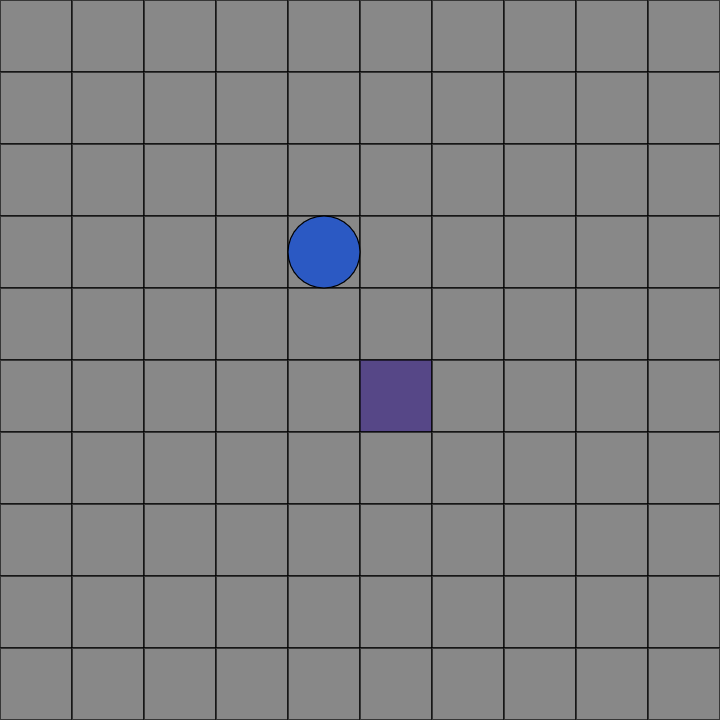
\includegraphics[scale=0.25]{app-labirint-imagine-cu-mutare}
	\caption{Reprezentarea vizual@a a labirintului dup@a o serie de ac@tiuni ale agentului}
	\label{fig:labirint-imagine-cu-mutare}
\end{figure}


\section{Simulator}

Simulatorul actioneaz@a ca o interfa@ta @intre agent @si mediul reprezentat de labirint. Acesta are rolul s@a furnizeze informa@tii c\^ atre agent, precum: codificarea curent@a a labirintului sau reprezentarea sa sub form@a de imagine; dac@a simularea este terminat@a; recompensa pentru fiecare ac@tiune luat@a.

Clasa \textbf{Env} este cea care define@ste structura modului de ac@tionare a simulatorului. Acesta define@ste trei func@tii principale, iar principiul lor de func@tionare este inspirat dup@a standardul definit de c\^ atre OpenAi Gym \cite{open-ai-gym-env-format}. A@sadar avem urm@atoarele func@tii:

\begin{itemize}
	\item reset - acest@a func@tie aduce mediul simulat la starea ini@tial@a (figura \ref{fig:labirint-imagine}) @si ruturnez@a aceast@a stare sub forma dorit@a (codificare sau imagine).
	\item step(ac@tiune) - aceasta transmite ac@tiunea luat@a de agent c\^ atre clasa \textbf{Board}, dup@a ac@tiunea este procesat@a, clasa \textbf{Board} transmite inapoi valoare recompensei al acelei ac@tiuni dac@a este valid@a, altfel doar anun@ta invaliditatea. Dupa preluarea rezultatului, se decide care este recompensa @si dac@a simularea s-a incheiat @in urma aceste ac@tiuni. Valorile noi starii, a recompensei @si a semnalului de terminare sunt returnate la finalul evalu@arii.
	\item actionSample - aceas@ta func@tie returneaz@a o ac@tiune aleatorie disponibil@a @in mediul simulat
\end{itemize}



\begin{lstlisting}[language=Java, caption=Definirea clasei Env]
class Env {
    ACTIONS = ['UP', 'DOWN', 'RIGHT', 'LEFT']
    invalidState = false
    /**
     * 
     * @param {Board} board 
     */
    constructor(board) {
        this.board = board
    }

    //
    setAgentStartPosition(pos) {
        this.board.playerDefaultPos = pos
    }

    // 
    step(action) {
        this.invalidState = !this.board.move(this.ACTIONS[action])
        return  this.board.getBoardState(), this._getReward(), this._isDone()]
    }

    //
    reset() {
        this.board.playerReset()
        return this.board.getBoardState()
    }

    //
    actionSample() {
        return Math.floor(Math.random() * this.ACTIONS.length)
    }

    //
    _getReward() {
        return (this.invalidState && !this.board.isOnExit() && -100) || this.board.getPlayerCellValue()
    }

    //
    _isDone() {
        return this.board.isOnExit() || this.invalidState
    }

    //
    clone() {
        return new Env(this.board.clone())
    }
}
\end{lstlisting}


\section{Agent}

Clasa \textbf{Agent} define@ste structura intern@a a re@telei neuronale. Pentru construirea re@teleor neuronale folosim biblioteca Tensorflow care ne ofer@a o multitudine de func@tii pentru definirea straturilor, a func@tilor de activare @si diverse metode de manipulare a datelor. Func@tiile din Tensorflow lucreaz@a @in principal cu valori reprezentate prin tensori defini@ti de clasa \texttt{Tensor} a bibliotecii. Monitorizarea num@arului de tensori crea@ti de-a lungul se\-si\-u\-ni\-lor de antrenament ale agentului are o desebit@a importan@t@a @in detectarea problemelor legate de consumul de resurse al calculatorului.

Func@tiile principale ale clasei sunt:
\begin{itemize}
	\item predict (date de intrare) - aceasta ne ofer@a rezultatul din urma proces@arii datelor de intrare oferite ca parametru
	\item fit(date de intrare, date de ie@sire) - aplic@a algoritmul de optimizare astfel @inc\^ at rezultatul datelor de intrare s@a fie cat mai aproape de rezultatul dorit definit @in datele de ie@sire date ca parametru
\end{itemize}

Pentru crearea re@telei neuronale vom folosii func@tia \texttt{sequential} care cere ca paremetri o list@a de str@aturi definite de pachetul \texttt{layers}. Cel mai important strat este cel de tip \texttt{dense}, care reprezint@a structura de baza al unui strat definit @in capitlul 2. Acesta este compus din ponderi sinaptice @si op@tional o func@tie de activare. Un exemplu de definire al unei simple re@tele neuronale cu un singur strat @si un singur neuron, f@ar@a func@tie de activare @si deplasare (bias), care accept@a un vector de valori de lungime 3 arat@a astfel:

\begin{lstlisting}[language=Java, caption={Exemplu de creare a unei rețele neuronale simple}]
import * as tf from '@tensorflow/tfjs';

const rn = tf.sequential();
rn.add( tf.layers.dense({ units: 1, inputShape: [3], useBias: false }) );
\end{lstlisting}

Func@tia de activare nu a fost specificat@a, iar deplasarea  (bias) a fost dezactivat@a, prin urmarea la evaluare vectorului se va afi@sa produsul scalar dintre vectorul cu datele de intrare @si vectorul ponderilor sinaptice. Formula arat@a astfel: $$rezultat = <(w_1, w_2, w_3),(x_1, x_2, x_3)> = w_1 * x_1 + w_2 * x_2 + w_3 * x_3  $$

Pentru evaluarea vectorului vom folosii func@tia \texttt{predict} definit@a de \texttt{sequential}. Este important s@a re@tinem faptul c@a \texttt{predict} trebuie s@a primeasc@a un vector de date de intrare, iar rezultatul s@au este un vector de date de i@sire. A@sadar, vectorul nostru de 3 elemente trebuie pus @intr-un alt vector, care @in final arat@a precum o matrice care va fi transformat @intr-un tensor 2-dimensional prin folosirea func@tiei \texttt{tensor2d}. Biblioteca Tensorflow lucreaz@a @in principal cu tensori, a@sa c@a este foarte important s@a transmitem datele @in formatul corect. Dac@a am fi avut o matrice ca date de intrare, atunci ar fi trebuit s@a cre@am un tensor 3-dimensional.
Ini@tieniera valorilor ponderilor sinaptice este aleatoare, @si pentru vizualizarea lor punem @in datele de intrare o valoarea cu 1 @si restul cu 0.

\begin{lstlisting}[language=Java, caption={Exemplu de evaluare a unei simple re@tele neuronale}]
// Afișează valoarea primei ponderi sinaptice
rn.predict(tf.tensor2d([[1, 0, 0]])).print(); // [[1.1913936],]
// Afișează valoarea pentru a doua pondere sinaptică
rn.predict(tf.tensor2d([[0, 1, 0]])).print(); // [[0.665537],]
// Afișează valoarea pentru a treia pondere sinaptică
rn.predict(tf.tensor2d([[0, 0, 1]])).print(); // [[-0.9657576],]
// Afișează suma celor trei ponderi sinaptice 
rn.predict(tf.tensor2d([[1, 1, 1]])).print(); // [[0.891173],]
\end{lstlisting}

Se poate observa c@a pe linia 8 se va afi@sa suma valorilor de pe liniile 2, 4, 6. Vom adauga o func@tie de activare @si anume \textit{relu} (Rectified Linear Unit), descris@a @in capitolul 2. Acesta func@tie de activare transforma valorile negative @in valoarea 0, astfel av\^ and un rol de filtrare a valorilor negative. Exemplu:

\begin{lstlisting}[language=Java, caption={Exemplu de evaluare a unei simple rețele neuronale cu funcție de activare}]
const rn = tf.sequential();
rn.add( tf.layers.dense({ units: 1, inputShape: [3], activation: "relu", useBias: false }) );
rn.predict(tf.tensor2d([[1, 0, 0]])).print(); // [[0.1161228],] 
rn.predict(tf.tensor2d([[0, 1, 0]])).print(); // [[0],]
rn.predict(tf.tensor2d([[0, 0, 1]])).print(); // [[0.3614732],]
rn.predict(tf.tensor2d([[1, 1, 1]])).print(); // [[0],]
\end{lstlisting}

Se observ@a faptul a doua pondere sinaptic@a are o valoarea negativ@a fa@t@a de celelalte dou@a, iar din linia 6, reiese faptul c@a aceasta este mult mai mare decat suma celorlalte dou@a, cea ce duce ca rezultatul final s@a fie 0. Interpretarea valorilor ob@tinute este un factor important @in in@telegerea re@telei neuronale. Din exempul anterior, a doua pondere sinaptic@a are o influen@ta mult mai mare asupra rezultatului dec\^ at restul. Dac@a dorim ca aceasta s@a aiba o influen@ta mult mai mica, trebuie s@a folosim procedeul de antrenare a re@telei care ne va calibra valorile acestor ponderi sinaptice, astel @inc\^ at s@a ob@tinem o valoare finala mult mai aproape de cea ce dorim.

Pentru antrenarea re@telei neuronale vom folosii func@tia \texttt{fit} din \texttt{sequential}. De asemenea, trebuie s@a alegem @si o un optimizator care va fi \texttt{adam}, iar pentru calculul erori vom folosii metoda celor mai mici p@atrate (mean square error). Vom folosii modelul anterior pentru exemplificare @si vom antrena re@teaua astfel @incat prima pondere sinaptic@a s@a fie cat mai aproape de 0 ca valoare.

\begin{lstlisting}[language=Java, caption={Exemplu de antrenare a unei simple rețele neuronale cu funcție de activare}]
const rn = tf.sequential();
rn.add( tf.layers.dense({ units: 1, inputShape: [3], activation: "liniar", useBias: false }) );
rn.predict(tf.tensor2d([[1, 0, 0]])).print(); // [[0.1678354],] 
// Adaug optimizatorul și funcția pentru calculul erorii
rn.compile({ loss: "meanSquaredError", optimizer: "adam" });
// Creez o funcție de antrenare care va încercă să modifice prima pondere 
// sinaptică în decursul a 500 de episoade/iterații
(async () => {
	for (let i = 0; i < 500; ++i) {
		await rn.fit(tf.tensor2d([[1, 0, 0]]), tf.tensor2d([[0]]));
	}
	// Afișez rezultatul antrenamentului
	rn.predict(tf.tensor2d([[1, 0, 0]])).print(); // [[0.0001513],]
})();
\end{lstlisting}

Av\^ and exemple anterioare ca exemplificare a func@tilor din biblioteca \texttt{Tensorflow}, punem construi strucura @si modul de func@tionare a clasei \texttt{Agent}.

\begin{lstlisting}[language=Java, caption={Structura clasei Agent}]
import * as tf from '@tensorflow/tfjs';

class Agent {
    constructor(model) {
        /**
         * Inițiez rețeaua neuronală
         * @type {tf.Sequential}
         */
        this.model = model || this.buildModel()
    }

    // Funcție care construiește rețeaua neuronală
    buildModel() {
        const model = tf.sequential() // Creare rețea
        // Adaug primul strat care va primii pixelii pixeli imaginii labirintului
        model.add(tf.layers.dense({ units: 25, inputShape: [25, 25], activation: 'relu' }))
        // Adaug un strat intermediar care îmi înlocuiește unele  
        // de date de intrare pentru următorul strat cu valoarea 0
        model.add(tf.layers.dropout({ rate: 0.4 }))
        // Un strat ascuns care va suma pe fiecare linie rezultatele anterioare
        model.add(tf.layers.dense({ units: 1, activation: 'relu' }))
        // Un strat intermediar care îmi va reduce dimensiunea, astfel din matrice toate
        // toate datele de intrare devin un singur vector
        model.add(tf.layers.flatten())
        model.add(tf.layers.dropout({ rate: 0.2 }))
        // Stratul final care ne oferii rezultatul sub forma unui vector de 4 elemente
        // ele reprezentând valoarea acțiunilor pentru stare dată
        model.add(tf.layers.dense({ units: 4, activation: 'linear' }))
        // Adaug optimizatorul și funcția de calcul a erorii
        model.compile({ loss: 'meanSquaredError', optimizer: 'adam', metrics: ['accuracy'] })
        return model
    }

    // Funcție de antrenare
    async fit(input, output) {
        await this.model.fit(input, output, { epochs: 1 })
    }
    
    // Funcție care evaluează datele de intrare
    predict(input) {
        return this.model.predict(input.expandDims(0))
    }
    
    // Funcție care evalueză datele de intrare și returnează
    // poziția pentru cel mai mare element din datele de ieșire procesate
    getAction(input) {
        return tf.tidy(() => {
            const result = this.predict(input)
            return tf.argMax(result, 1).arraySync()[0]
        })
    }
}

export default Agent
\end{lstlisting}

\section{Model de @inv@a@tare}

Pentru implementarea modelul de @inv@a@tare vom folosii algoritmul Q-Learning descris @in capitolul 3. Vom avea nevoie de 3 clase principale: \texttt{Agent}, \texttt{Env} @si \texttt{Memory}.

Clasa \texttt{Memory} va fi cea care va pastra rezultatele experien@telor pe care agentul le va produce de-a lungul sesiunii de antrenament. Memoria va consta dintr-o lista de lungime data @in care se vor adauga experien@tele, daca se va dep@a@sii capacitatea, atunci experien@tele vechi for fi @sterse. Structura clasei \texttt{Memory} arat@a astfel:

\begin{lstlisting}[language=Java, caption={Structura clasei Memory}]
class Memory {
    constructor(capacity, cleanFun) {
        // Setare capacitate maximă
        this.capacity = capacity || 5000
        // Inițiere listă
        this.experiences = []
        // Setare funcție de curățare a memoriei fizice pentru valorile care vor fi distruse
        this.cleanFun = cleanFun
    }

    // Funcție care adaugă o experiență în listă
    add(exper) {
        // Verific dacă am depășit capacitatea
        if (this.experiences.length + 1 > this.capacity) {
            // Scot elementul vechi din listă
            const exper = this.experiences.shift()
            // Curăț elementul din memoria fizică
            this.cleanFun?.(exper)
        }
        // Adaug nouă experiență
        this.experiences.push(exper)
    }

    // Preiau o serie fixă de experiențe amestecate aleatoriu din lista
    sample(batch) {
        // Amestec toate experiențele
        const randomExperiences = Memory.shuffle([...this.experiences])
        // Preiau primele experiențe ca serie
        return randomExperiences.slice(0, batch)
    }

    // Golosesc toată lista de experiențe
    clean() {
        // Aplic funcție de curățare a memorie fizice
        // că să nu am posibile reziduri
        this.experiences.forEach(exper => {
            this.cleanFun?.(exper)
        })
        this.experiences = []
    }

    // Amestec o copie a unui vector dat folosind algoritmul Fisher-Yates
    static shuffle(array) {
        // Inițiere variabile
        let m = array.length, t, i;
        // Cât timp mai sunt elemente de amestecat
        while (m) {
            // Iau o poziție aleatorie
            i = Math.floor(Math.random() * m--);
            // Fac schimb de poziții cu elementul din poziția m
            t = array[m];
            array[m] = array[i];
            array[i] = t;
        }
        return array;
    }
}

export default Memory
\end{lstlisting}

Toate aceste piese vor fi folosite @in clasa \texttt{Trainer}, pentru crearea programului final de implementare al modelului de @inv@a@tare. Aceast@a clasa aplica algoritmul de Q-Learning (descris @in capitolul 3) pentru antrenarea re@telei neuronale al agentului descris@a de clasa \texttt{Agent}.

\begin{lstlisting}[language=Java, caption={Structura clasei Trainer}]
class Trainer {
    totalEnvs = 2
    /**
     * Inițiere componente
     * @param {Env} env 
     * @param {Agent} agent 
     * @param {Memory} memory
     */
    constructor(env, agent, memory) {
        // Setare memorie
        this.env = env
        // Setare agent
        this.agent = agent
        // Setare memorie
        this.memory = memory
        // Inițiere listă de simulatoare
        this.envs = [{ id: 1, env: this.env }]
    }

    async train(episodes = 150, cb = () => { }) {
        const discount = 0.985; // Factor de atenuare
        // const lr = 0.1
        let epsilon = 1 // Probailitatea unei acțiuni aleatoare
        const epsilon_min = 0.0 // Probailitatea minimă a unei acțiuni aleatoare
        const epsilon_decay = (epsilon - epsilon_min) / episodes // Rata de scădere a probabilității
        const maxIterations = 75 // Numărul de iterații maxime

        // Simulări episod
        for (let eps = 1; eps <= episodes; eps++) {
        
            const t0 = performance.now() // Timpul de incepere
            const rewardsAnaly = {} // Obiecte cu date de tip analitic
            // Rulare simulării unui episod în fiecare simulator înregistrat în listă
            await Promise.all(this.envs.map(async ({ id, env }) => {
                // Re-inițiere simulator și prealuarea stării de început
                let state = await env.reset()

                // Rulare simulare
                for (let iter = 0; iter < maxIterations; iter++) {
                    // Alegerea acțiunii
                    const action = Math.random() < epsilon ? env.actionSample() : this.agent.getAction(state)
                    // Procesarea acțunii și colectarea rezultatului
                    const [nextState, reward, done] = await env.step(action)
                    // Salvare în memorie
                    this.memory.add({ state, nextState, reward, done, action })

                    // Sumarea recompenselor adunate pe parcursul episodului
                    rewardsAnaly[id] = rewardsAnaly[id] ? rewardsAnaly[id] + reward : reward
                    // Oprire simulare în cazul semnalului de stop
                    if (done) {
                        break
                    }
                    // Prealuare stării viitoare
                    state = nextState
                }
            }))

            const tData = performance.now() // Timpul de începere a procesării de date

            // Alegerea a 100 de experiențe aleatoare și procesarea lor
            const trainData = this.memory.sample(100).filter(exper => !exper.state.isDisposed && !exper.nextState.isDisposed).reduce((acc, exper) => {
                return tf.tidy(() => {
                    // Preiau datele din experiență
                    const { nextState, reward, done, state, action } = exper
                    // Calculez valoare Q pentru viitoare stare
                    const nextQ = (this.agent.predict(nextState).arraySync())[0]
                    // Calculez valoarea Q curentă
                    const newCurrentQ = (this.agent.predict(state).arraySync())[0]
                    // Aplic ecuația Bellman
                    newCurrentQ[action] = done ? reward : reward + discount * Math.max(...nextQ)
                    // Salvez rezultatele
                    acc.states.push(state);acc.newQValues.push(newCurrentQ)
                    return acc
                })

            }, { states: [], newQValues: [] })

            const tTrain = performance.now() // Timpul de începere al antrenării rețelei neuronale
            await this.agent.fit(tf.stack(trainData.states), tf.tensor2d(trainData.newQValues))
            const tEnd = performance.now() // Timpul de sfărsit de episod

            // Reduc probilitatea în funcție de rata sa 
            if (epsilon > epsilon_min) {
                epsilon -= epsilon_decay
                epsilon = Math.max(epsilon, 0)
            }

            // Trimit datele analitice către interfața de utilizator 
            cb({
                episode: eps, // Numărul episodului
                episodeTime: tEnd - t0, // Durata episodului
                dataPreparation: tTrain - tData, // Durata procesării de date
                fitDuration: tEnd - tTrain, // Durata de antrenament a    rețelei
                episodeRewards: rewardsAnaly, // Recompensele acumulate
                numTensors: tf.memory().numTensors, // Numărul de tensori
                numBytes: tf.memory().numBytes // Spațiul de memorie ocupat
            })

            // La fiecare 50 de episoade curăț toată memoria
            if (eps % 50 === 0 && eps > 1) {
                console.log('CLEAN ALL MEMORY', eps)
                this.memory.clean()
            }
        }
        // Semnalez că antrenamentul s-a încheiat
        return 'completed'
    }
}
export default Trainer
\end{lstlisting}

Av\^ and implementarea tuturor claselor necesare, o sesiune de antrenament poate fi ini@tiat@a astfel:

\begin{lstlisting}[language=Java, caption={Inițierea unei sesiuni complete de antrenament}]
 // Inițiere labirint
 const board = new Board(10, 10);
 // Inițieri reprezentare vizuală a labirintului
 const boardUI = new BoardUI(board, new Konva.Stage({
	container: "container",
	width: 600,
	height: 600,
 }));
 // Inițiere simulator
 const env = new ImageEnv(board, boardUI);
 // Inițiere agent
 const agent = new ImageAgent();
 // Inițiere memorie
 const memory = new Memory(100, cleanMemoryExperience);
 // Inițiere mediu de antrenare
 const trainer = new ImageTrainer(env, agent, memory);
 // Inițiere sesiune de antrenament
 trainer.train()
\end{lstlisting}

Av\^ and programul complet, vom folosii datele analitice furnizate pentru crearea unei interfe@te interactive pentru utilizator. Aceste poate vedea durata antrenamentului, performan@ta dob\^ andit@a de-a lungul sesiunilor, etc.

\section{Interfa@t@a Utilizator}

Toata aplic@tia este conceput@a ca un site web, iar marele avantaj al acestui lucru este c@a putem dezvolta o interfa@t@a interactiv@a complex@a destinat@a utilizatorului, @in care poate interac@tiona foarte u@sor cu modele de @inv@a@tare @si vizualiza datele rezultatele folosind grafice care sunt actualizate @intr-un timp extrem de scurt.

Dup@a ini@tierea aplica@tiei, va aparea o imagine cu reprezentarea grafic@a a labirintului prin clasa \texttt{BoardUI} @si un tabel care prezint@a codificarea sa dat de clasa \texttt{Board}. Pentru ini@tierea agentului trebuie s@a apas@am pe butonul \textsl{Ini@tializeaz@a un now agent}.

Odat@a ap@a
sat butonul, observ@am ca am avem disponibile urm@atoarele butoane:
\begin{itemize}
	\item Atrenare - buton care ini@tializeaz@a sesiunea de antrenament
	\item Rulare - buton care ini@tiaz@a o sesiune de test pentru observarea progresului
	\item Reset - buton care aduce labirintul la starea ini@tial@a
\end{itemize}

Pe lang@a aceste butoane, avem @si op@tiuni care ne permite s@a modific@am pozi@tia agentului cu ajutorlul mouse-lui sau s@a ad@aug@am un obstacol in labirint. @In dreapta labirintului sunt prezente etichete care ne arat@a dac@a agentul se afl@a @intr-o sesiune de antrenament, informa@tii legate de valoare ac@tiunilor din pozi@tia curent@a a agentului @in labirin @si un camp de date care ne permite s@a introducem num@arul de episoade al sesiunii de antrenament.

Dac@a ap@as@am pe butonul \textsl{Rulare}, observam un comportament aleatoriu din partea agentului, deoarece re@teauna neuronal@a nu este atrenat@a, iar valorile ponderilor sinaptice au fost ini@tiate aleatoriu.

Odat@a ap@asat pe botonul \textsl{Antrenare}, observ@am c@a avem noi elemente vizuale. Acestea sunt cele care vor con@tine date despre performan@ta agentului @si al sesiunii de antrenament.  
\addcontentsline{toc}{chapter}{Concluzii finale}

\markboth{\bf Concluzii finale}{\bf Concluzii finale}

%% capitolul de concluzii
%%
%%
\chapter*{Concluzii finale}

\markboth{\bf Concluzii finale}{\bf Concluzii finale}


\^ In aceast\u a lucrare am analizat cum elementele de @inv@a@tare automat@a (re@tele neuronale, Q-Learning) ajut@a la abordarea de probleme complexe, precum antrenarea de agent@i autonomi care s@a @indeplineasc@a obiectivele date @in constr\^ angerile din mediul de lucru. Folosind biblioteca Tensflow am ar@arat cum putem face un prototip pentru agent care poate s@a parcurg@a un labirint pentru a ajunge la o pozi@tie dorit@a. 

Partea complex@a pentru rezolvarea sarcinei este procesarea datelor de intrare care sunt sub form@a de imagini. Dac@a am fi ales s@a rezolv@am aceast@a problem@a @intr-o manier@a clasic@a, @si anume prin analiza imaginior folosind tehnici de prelucrare a imaginilor (filtre pentru detectarea de muchii, analiza formelor geometrice) @si apoi transformarea lor @intr-un graf care s@a reprezinte modul de modelare al mediului simulat. Apoi a aplicat un algoritm care s@a ne ofere traseul pan@a la obiectiv.

Utiliz@and re@tele neuronale nu am avut nevoie de o analiz@a asupra imaginilor sau a modului cum func@tioneaz@a simularea la ini@tiere, deoarece aceasta vor deduse de c@atre algoritmul Q-Learning pe parcursul procesului de antrenare care folo@ste de recompensele acumulate de agent @in urma ac@tiunilor sale pentru a stabilii care sunt cele mai bune decizii pentru fiecare situa@tie.

Folosind interfa@ta dedicat@a utlizatorului am putut observ@a cum decurge o sesiune de antrenament, cum se @imbun@at@a@tesc decizii date de re@tea, volumul de resurse consumate @si timpul necesar al @intregii opera@tiuni.
\index{concluzii}